\section{解的误差与敏感性}
\label{sec:ls-numerical-sensitivity}

求解目标确定、算法也给出结果以后，还要回答算出的结果能相信多少。本节分四方面讨论：数据的扰动怎样传到解，算出的近似解怎样用残差判断，最小二乘的不同输出各有多敏感，以及矩阵的秩变化时伪逆怎样变化。

讨论每种误差，都要先说清以什么为参照、允许修改哪些数据。比较两个精确解时，修改的是$\bm A$或$\bm b$，参照是原问题的精确解。用残差判断近似解时，数据不改，参照是未知的真解。后向误差则反过来问：数据至少要改多少，近似解才成为修改后问题的精确解。

以下结论都由精确方程、范数估计和奇异值性质建立，扰动可以有有限大小；所用的条件数与奇异值扰动界来自第~\ref{chap:condition-and-spectral-perturbation}章。扰动趋于零时的局部观点留到后文：第~\ref{chap:matrix-differentiation}章建立逆矩阵等运算的微分公式，第~\ref{chap:differential-perturbation-analysis}章再从同样的精确关系中提取解映射的一阶响应，讨论局部条件数与一阶近似的余项。

\subsection{系数矩阵与右端项的扰动}
\label{sec:ls-equation-sensitivity}

方程的数据常常来自测量或前一步计算，本身就带有误差。本小节回答：数据改变一点，方程的精确解改变多少。这里比较的是两个精确解，与算法和舍入无关，所以放大完全来自问题本身。

本小节设$\bm A\in\mathbb R^{d\times d}$可逆，$\bm b\ne\bm0$，精确解为$\bm x_\star=\bm A^{-1}\bm b$。向量范数与它诱导的矩阵范数始终取同一种，记
\[
 \kappa(\bm A)=\lVert\bm A\rVert\,\lVert\bm A^{-1}\rVert .
\]
用二范数时写作$\kappa_2(\bm A)$。

\paragraph{右端扰动}
先固定$\bm A$，只把右端改为$\bm b+\Delta\bm b$，记新解为$\bm x_\star+\Delta\bm x$。我们关心的是解的相对变化与右端的相对变化之比，它说明右端的误差被放大了多少倍。

新旧两个方程分别为
\[
 \bm A(\bm x_\star+\Delta\bm x)=\bm b+\Delta\bm b,\qquad \bm A\bm x_\star=\bm b .
\]
两式相减，得到
\begin{equation}
 \bm A\,\Delta\bm x=\Delta\bm b,\qquad\text{即}\qquad \Delta\bm x=\bm A^{-1}\Delta\bm b .
 \label{eq:ls-rhs-perturbation-exact}
\end{equation}
推导中没有任何近似，所以这个关系对任意大小的$\Delta\bm b$都精确成立。

对它取范数，得到解的绝对变化的界
\[
 \lVert\Delta\bm x\rVert\leq\lVert\bm A^{-1}\rVert\,\lVert\Delta\bm b\rVert .
\]
要换成相对变化，还需要用$\lVert\bm b\rVert$估计$\lVert\bm x_\star\rVert$。由$\bm b=\bm A\bm x_\star$，
\[
 \lVert\bm b\rVert\leq\lVert\bm A\rVert\,\lVert\bm x_\star\rVert,\qquad\text{即}\qquad \frac1{\lVert\bm x_\star\rVert}\leq\frac{\lVert\bm A\rVert}{\lVert\bm b\rVert}.
\]
两个不等式相乘，得到相对误差界
\begin{equation}
 \frac{\lVert\Delta\bm x\rVert}{\lVert\bm x_\star\rVert}\leq\kappa(\bm A)\,\frac{\lVert\Delta\bm b\rVert}{\lVert\bm b\rVert}.
 \label{eq:ls-rhs-relative-error-bound}
\end{equation}
这就是第~\ref{sec:ls-matrix-condition-number}节的条件数界（定理~\ref{thm:matrix-analysis-condition-number-bound}）：条件数是右端相对误差的最大放大倍数。

哪些方向上的右端误差放大得最多，可以由奇异值分解读出。设$\bm A=\sum_{i=1}^d\sigma_i\bm u_i\bm v_i^\top$，把右端的变化按左奇异向量展开，
\[
 \Delta\bm b=\sum_{i=1}^d\beta_i\bm u_i,\qquad \beta_i=\bm u_i^\top\Delta\bm b .
\]
由于$\bm A^{-1}=\sum_i\sigma_i^{-1}\bm v_i\bm u_i^\top$，解的变化为
\begin{equation}
 \Delta\bm x=\bm A^{-1}\Delta\bm b=\sum_{i=1}^d\frac{\beta_i}{\sigma_i}\,\bm v_i .
 \label{eq:ls-rhs-perturbation-svd}
\end{equation}
沿$\bm u_i$的误差分量被放大$1/\sigma_i$倍，并转到$\bm v_i$方向上。误差落在最小奇异值对应的方向上时，放大最多。下面的例子在精确算术中计算，比较一个良态矩阵和一个两列接近同向的矩阵。

\begin{example}[良态矩阵与近平行列矩阵]
\label{ex:ls-rhs-perturbation-near-parallel}
先看一个良态的对照，取以下数据：
\[
 \bm A_1=\begin{bmatrix}2&0\\0&1\end{bmatrix},\qquad \bm b=\begin{bmatrix}2\\1\end{bmatrix}.
\]
精确解为$\bm x_\star=(1,1)^\top$，$\kappa_2(\bm A_1)=2$。把右端的第二个分量改为$1.01$，即$\Delta\bm b=(0,0.01)^\top$，则解的变化为
\[
 \Delta\bm x=\bm A_1^{-1}\Delta\bm b=\begin{bmatrix}0\\0.01\end{bmatrix},
\]
新解为$(1,1.01)^\top$。右端与解的相对变化分别为
\[
 \frac{\lVert\Delta\bm b\rVert_2}{\lVert\bm b\rVert_2}=\frac{0.01}{\sqrt5}\approx0.00447,\qquad
 \frac{\lVert\Delta\bm x\rVert_2}{\lVert\bm x_\star\rVert_2}=\frac{0.01}{\sqrt2}\approx0.00707,
\]
放大约$1.58$倍，不超过$\kappa_2(\bm A_1)=2$。

再取两列接近同向的矩阵
\[
 \bm A_2=\begin{bmatrix}1&1\\0&\varepsilon\end{bmatrix},\qquad \varepsilon=10^{-2},
\]
它的逆矩阵为
\[
 \bm A_2^{-1}=\begin{bmatrix}1&-1/\varepsilon\\0&1/\varepsilon\end{bmatrix}.
\]
右端取$\bm b=(2,0)^\top$，解为$\bm x_\star=(2,0)^\top$。把右端的第二个分量改为$\eta$，解的变化按元素为
\[
 \Delta\bm x=\bm A_2^{-1}\begin{bmatrix}0\\\eta\end{bmatrix}=\begin{bmatrix}-\eta/\varepsilon\\\eta/\varepsilon\end{bmatrix}.
\]
取$\eta=0.01$，得$\Delta\bm x=(-1,1)^\top$，解由$(2,0)^\top$变为$(1,1)^\top$。右端与解的相对变化分别为
\[
 \frac{\lVert\Delta\bm b\rVert_2}{\lVert\bm b\rVert_2}=\frac{0.01}{2}=0.005,\qquad
 \frac{\lVert\Delta\bm x\rVert_2}{\lVert\bm x_\star\rVert_2}=\frac{\sqrt2}{2}\approx0.707,
\]
放大约$141$倍。

这个倍数可以与条件数比较。$\bm A_2^\top\bm A_2=\left[\begin{smallmatrix}1&1\\1&1+\varepsilon^2\end{smallmatrix}\right]$的特征值是$\sigma_{\max}^2$与$\sigma_{\min}^2$，由迹与行列式得
\[
 \sigma_{\max}^2+\sigma_{\min}^2=2+\varepsilon^2,\qquad \sigma_{\max}\sigma_{\min}=\varepsilon .
\]
解出
\[
 \sigma_{\max}\approx1.41423,\qquad \sigma_{\min}\approx0.0070710,
\]
所以$\kappa_2(\bm A_2)\approx200$。

实际倍数$141$没有达到$200$，差别来自$\bm b$：界中用$\lVert\bm A_2\rVert_2\approx1.414$估计$\lVert\bm b\rVert_2/\lVert\bm x_\star\rVert_2$，而这里该比值为$1$。

放大的方向也可以由奇异向量看出。数值计算给出
\[
 \bm v_{\min}\approx\begin{bmatrix}0.7071\\-0.7071\end{bmatrix},\qquad
 \bm u_{\min}\approx\begin{bmatrix}0.0050\\-1.0000\end{bmatrix}.
\]
$\Delta\bm b=(0,0.01)^\top$几乎全部落在$\bm u_{\min}$上，系数$\beta_{\min}\approx-0.0100$，而沿另一方向的系数只有约$5\times10^{-5}$。于是
\[
 \Delta\bm x\approx\frac{\beta_{\min}}{\sigma_{\min}}\,\bm v_{\min}\approx-1.4142\,\bm v_{\min}\approx\begin{bmatrix}-1\\1\end{bmatrix}.
\]
解的变化正沿着$\bm v_{\min}$，两个系数此增彼减。图~\ref{fig:matrix-analysis-coefficient-sensitivity}画出了$\varepsilon$减小时这种分裂怎样加剧。
\end{example}

\begin{figure}
 \centering
 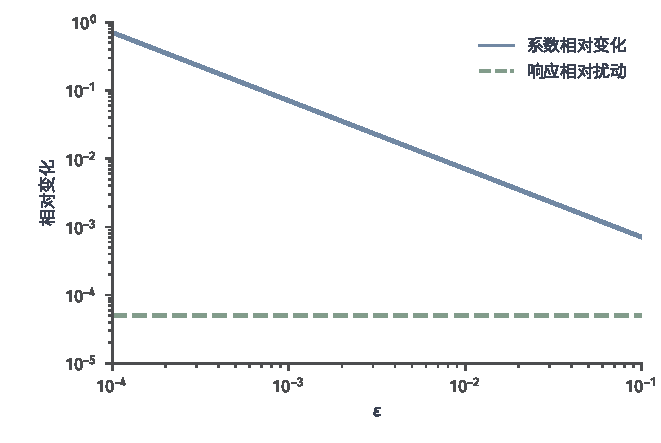
\includegraphics[width=0.92\linewidth]{figures/00-shared/mathematical-preliminaries-upper/02-linear-spaces/matplotlib/matrix-analysis-coefficient-sensitivity/figure.pdf}
 \caption{近平行列的系数分裂。取$\bm A_2=\left[\begin{smallmatrix}1&1\\0&\varepsilon\end{smallmatrix}\right]$、$\bm b=(2,0)^\top$，固定右端扰动$\Delta\bm b=(0,10^{-4})^\top$。蓝线为系数相对变化$\lVert\Delta\bm x\rVert_2/\lVert\bm x\rVert_2$，绿虚线为右端相对扰动$\lVert\Delta\bm b\rVert_2/\lVert\bm b\rVert_2$。两个系数沿相反方向偏离$(2,0)^\top$，变化量随$1/\varepsilon$增长。}
 \label{fig:matrix-analysis-coefficient-sensitivity}
\end{figure}

\paragraph{系数矩阵的扰动}
\label{sec:ls-inverse-sensitivity}%
系数矩阵的元素也可能带误差。设扰动后的矩阵为$\bm B=\bm A+\bm E$。与右端扰动不同，这时会出现一个新问题：$\bm B$甚至可能不可逆，例如$\bm E=-\bm A$。所以要先确定扰动多小时$\bm B$一定可逆，再估计$\bm B^{-1}$离$\bm A^{-1}$多远。

直观地看，$\bm E$是否算“小”，不能只看它本身的大小，还要看$\bm A$离奇异有多远。$\bm A^{-1}$的范数越大，$\bm A$越接近奇异，能容忍的扰动越小。下面的定理用乘积$\bm A^{-1}\bm E$或$\lVert\bm A^{-1}\rVert\lVert\bm E\rVert$来衡量扰动。

\begin{theorem}[逆矩阵的有限扰动]
\label{thm:ls-inverse-finite-perturbation}
设$\bm A\in\mathbb R^{d\times d}$可逆，$\bm B=\bm A+\bm E$。
\begin{enumerate}
 \item 若$\lVert\bm A^{-1}\bm E\rVert<1$，则$\bm B$可逆，
 \begin{equation}
  \lVert\bm B^{-1}\rVert\leq\frac{\lVert\bm A^{-1}\rVert}{1-\lVert\bm A^{-1}\bm E\rVert},
  \label{eq:ls-inverse-norm-bound}
 \end{equation}
 且
 \begin{equation}
  \bm B^{-1}-\bm A^{-1}=-\bm B^{-1}\bm E\,\bm A^{-1}.
  \label{eq:ch06-inverse-finite-perturbation}
 \end{equation}
 \item 若$q=\lVert\bm A^{-1}\rVert\lVert\bm E\rVert<1$，则第1条适用，并且
 \begin{equation}
  \frac{\lVert\bm B^{-1}-\bm A^{-1}\rVert}{\lVert\bm A^{-1}\rVert}
  \leq\frac{q}{1-q},\qquad q=\kappa(\bm A)\frac{\lVert\bm E\rVert}{\lVert\bm A\rVert}.
  \label{eq:ls-inverse-relative-perturbation-bound}
 \end{equation}
\end{enumerate}
\end{theorem}
\begin{proof}
先证第1条中的可逆性。设$\bm B\bm x=\bm0$，即$\bm A\bm x=-\bm E\bm x$，两边左乘$\bm A^{-1}$并取范数，
\[
 \bm x=-\bm A^{-1}\bm E\bm x,\qquad \lVert\bm x\rVert\leq\lVert\bm A^{-1}\bm E\rVert\,\lVert\bm x\rVert .
\]
由于$\lVert\bm A^{-1}\bm E\rVert<1$，只能$\lVert\bm x\rVert=0$。方阵$\bm B$的零空间只含零向量，故$\bm B$可逆。

再估计$\lVert\bm B^{-1}\rVert$。对任意$\bm y$，令$\bm x=\bm B^{-1}\bm y$，则$\bm A\bm x+\bm E\bm x=\bm y$。左乘$\bm A^{-1}$并取范数，
\[
 \begin{gathered}
 \bm x=\bm A^{-1}\bm y-\bm A^{-1}\bm E\bm x,\\
 \lVert\bm x\rVert\leq\lVert\bm A^{-1}\rVert\,\lVert\bm y\rVert+\lVert\bm A^{-1}\bm E\rVert\,\lVert\bm x\rVert .
 \end{gathered}
\]
把含$\lVert\bm x\rVert$的项移到左边，
\[
 \bigl(1-\lVert\bm A^{-1}\bm E\rVert\bigr)\lVert\bm B^{-1}\bm y\rVert\leq\lVert\bm A^{-1}\rVert\,\lVert\bm y\rVert .
\]
对所有$\lVert\bm y\rVert=1$取上确界，即得$\lVert\bm B^{-1}\rVert$的界。恒等式由$\bm A-\bm B=-\bm E$得到：
\[
 \begin{aligned}
 \bm B^{-1}-\bm A^{-1}&=\bm B^{-1}\bm A\bm A^{-1}-\bm B^{-1}\bm B\bm A^{-1}\\
 &=\bm B^{-1}(\bm A-\bm B)\bm A^{-1}=-\bm B^{-1}\bm E\bm A^{-1}.
 \end{aligned}
\]

第2条中，$\lVert\bm A^{-1}\bm E\rVert\leq\lVert\bm A^{-1}\rVert\lVert\bm E\rVert=q<1$，所以第1条适用，并有$\lVert\bm B^{-1}\rVert\leq\lVert\bm A^{-1}\rVert/(1-q)$。对式~\eqref{eq:ch06-inverse-finite-perturbation}取范数，
\[
 \begin{aligned}
 \lVert\bm B^{-1}-\bm A^{-1}\rVert&\leq\lVert\bm B^{-1}\rVert\,\lVert\bm E\rVert\,\lVert\bm A^{-1}\rVert\\
 &\leq\frac{\lVert\bm A^{-1}\rVert^2\lVert\bm E\rVert}{1-q}=\frac{q}{1-q}\,\lVert\bm A^{-1}\rVert .
 \end{aligned}
\]
两边除以$\lVert\bm A^{-1}\rVert$即得。最后，
\[
 q=\lVert\bm A\rVert\lVert\bm A^{-1}\rVert\cdot\frac{\lVert\bm E\rVert}{\lVert\bm A\rVert}=\kappa(\bm A)\frac{\lVert\bm E\rVert}{\lVert\bm A\rVert}.
\]
\end{proof}

界的分子$q$是条件数乘矩阵的相对扰动，分母$1-q$是到可逆性保证边界的余量。$q$越接近$1$，余量越小，界就越大。

\begin{example}[一次系数扰动]
\label{ex:ls-inverse-perturbation-numeric}
取示例~\ref{ex:ls-stationary-running-example}的矩阵，并只扰动它的右下角元素：
\[
 \bm A=\begin{bmatrix}4&1\\1&3\end{bmatrix},\qquad
 \bm E=\begin{bmatrix}0&0\\0&1/2\end{bmatrix}.
\]
扰动后的矩阵为
\[
 \bm B=\bm A+\bm E=\begin{bmatrix}4&1\\1&7/2\end{bmatrix}.
\]
两个逆矩阵分别为
\[
 \bm A^{-1}=\frac1{11}\begin{bmatrix}3&-1\\-1&4\end{bmatrix},\qquad
 \bm B^{-1}=\frac1{26}\begin{bmatrix}7&-2\\-2&8\end{bmatrix}.
\]
直接相减，得
\[
 \bm B^{-1}-\bm A^{-1}=\frac1{286}\begin{bmatrix}-1&4\\4&-16\end{bmatrix}.
\]
按恒等式~\eqref{eq:ch06-inverse-finite-perturbation}计算$-\bm B^{-1}\bm E\bm A^{-1}$，得到同一个矩阵。它是一个秩一矩阵，
\[
 \bm B^{-1}-\bm A^{-1}=-\frac1{286}\begin{bmatrix}1\\-4\end{bmatrix}\begin{bmatrix}1&-4\end{bmatrix},
\]
谱范数为$17/286\approx0.0594$。

在谱范数下，$\bm A$的特征值为$(7\pm\sqrt5)/2$，所以
\[
 \lVert\bm A\rVert_2\approx4.618,\qquad \lVert\bm A^{-1}\rVert_2\approx0.4198,\qquad \kappa_2(\bm A)\approx1.939 .
\]
于是
\[
 q=\lVert\bm A^{-1}\rVert_2\lVert\bm E\rVert_2\approx0.4198\times0.5\approx0.210 .
\]
定理给出的界与实际的相对变化分别为
\[
 \frac{q}{1-q}\approx0.266,\qquad
 \frac{\lVert\bm B^{-1}-\bm A^{-1}\rVert_2}{\lVert\bm A^{-1}\rVert_2}\approx\frac{0.0594}{0.4198}\approx0.142 .
\]
第1条的范数界也成立。这里
\[
 \lVert\bm A^{-1}\bm E\rVert_2=\frac{\sqrt{17}}{22}\approx0.187,
\]
界为$0.4198/(1-0.187)\approx0.517$，而$\lVert\bm B^{-1}\rVert_2\approx0.368$。
\end{example}

这个界可以取到。取对角矩阵
\[
 \bm A=\begin{bmatrix}1&0\\0&\varepsilon\end{bmatrix},\qquad
 \bm E=\begin{bmatrix}0&0\\0&-\delta\end{bmatrix},\qquad 0<\delta<\varepsilon<1 .
\]
在谱范数下$\lVert\bm A^{-1}\rVert_2=1/\varepsilon$，$q=\delta/\varepsilon$。逆矩阵只在右下角改变，
\[
 \bm B^{-1}-\bm A^{-1}=\begin{bmatrix}0&0\\0&\dfrac1{\varepsilon-\delta}-\dfrac1\varepsilon\end{bmatrix}.
\]
右下角元素等于$\delta/(\varepsilon(\varepsilon-\delta))$，所以相对变化为
\[
 \frac{\lVert\bm B^{-1}-\bm A^{-1}\rVert_2}{\lVert\bm A^{-1}\rVert_2}=\frac{\delta}{\varepsilon-\delta}=\frac q{1-q}.
\]
例如$\varepsilon=0.1$、$\delta=0.05$时，$q=0.5$，逆矩阵的相对变化恰为$1$；$\delta\to\varepsilon$时它无界，因为$\bm B$趋于奇异。

反过来，$q\geq1$只表示定理不再给出保证，并不意味着$\bm B$已经奇异。例如$\bm E=\bm A$时$q=\kappa(\bm A)\geq1$，而$\bm B=2\bm A$仍可逆。

\paragraph{矩阵与右端同时扰动}
实际问题中矩阵与右端往往同时带误差。这时扰动后的方程为
\[
 (\bm A+\bm E)(\bm x_\star+\Delta\bm x)=\bm b+\Delta\bm b .
\]
展开左边，得
\[
 \bm A\bm x_\star+\bm A\Delta\bm x+\bm E\bm x_\star+\bm E\Delta\bm x=\bm b+\Delta\bm b .
\]
减去原方程$\bm A\bm x_\star=\bm b$，整理得到精确关系
\begin{equation}
 (\bm A+\bm E)\Delta\bm x=\Delta\bm b-\bm E\bm x_\star .
 \label{eq:ls-joint-perturbation-exact}
\end{equation}

式~\eqref{eq:ls-joint-perturbation-exact}说明，解的变化由两部分驱动：一是右端的变化$\Delta\bm b$，二是矩阵的变化作用在原解上产生的$\bm E\bm x_\star$。在定理~\ref{thm:ls-inverse-finite-perturbation}的条件下$\bm A+\bm E$可逆，于是
\[
 \Delta\bm x=(\bm A+\bm E)^{-1}(\Delta\bm b-\bm E\bm x_\star).
\]
下面的定理把两类扰动的相对大小合起来，估计解的相对变化。

\begin{theorem}[矩阵与右端同时扰动时的解误差]
\label{thm:ls-linear-system-perturbation}
设$\rho_A=\lVert\bm E\rVert/\lVert\bm A\rVert$，$\rho_b=\lVert\Delta\bm b\rVert/\lVert\bm b\rVert$。若$\kappa(\bm A)\rho_A<1$，则$\bm A+\bm E$可逆，且
\begin{equation}
 \frac{\lVert\Delta\bm x\rVert}{\lVert\bm x_\star\rVert}
 \leq\frac{\kappa(\bm A)\,(\rho_A+\rho_b)}{1-\kappa(\bm A)\rho_A}.
 \label{eq:matrix-analysis-linear-system-perturbation}
\end{equation}
\end{theorem}
\begin{proof}
由于$\kappa(\bm A)\rho_A=\lVert\bm A^{-1}\rVert\lVert\bm E\rVert$，可逆性由定理~\ref{thm:ls-inverse-finite-perturbation}第2条得到。把式~\eqref{eq:ls-joint-perturbation-exact}中的$\bm E\Delta\bm x$移到右边，再左乘$\bm A^{-1}$，
\[
 \Delta\bm x=\bm A^{-1}\bigl(\Delta\bm b-\bm E\bm x_\star-\bm E\Delta\bm x\bigr).
\]
取范数，得
\[
 \lVert\Delta\bm x\rVert\leq\lVert\bm A^{-1}\rVert\bigl(\lVert\Delta\bm b\rVert+\lVert\bm E\rVert\lVert\bm x_\star\rVert+\lVert\bm E\rVert\lVert\Delta\bm x\rVert\bigr).
\]
把含$\lVert\Delta\bm x\rVert$的项移到左边，
\[
 \begin{aligned}
 &\bigl(1-\lVert\bm A^{-1}\rVert\lVert\bm E\rVert\bigr)\lVert\Delta\bm x\rVert\\
 &\qquad\leq\lVert\bm A^{-1}\rVert\,\lVert\Delta\bm b\rVert+\lVert\bm A^{-1}\rVert\,\lVert\bm E\rVert\,\lVert\bm x_\star\rVert .
 \end{aligned}
\]
右边两项分别估计。由$\lVert\bm b\rVert\leq\lVert\bm A\rVert\lVert\bm x_\star\rVert$，
\[
 \begin{gathered}
 \lVert\bm A^{-1}\rVert\,\lVert\Delta\bm b\rVert=\lVert\bm A^{-1}\rVert\,\rho_b\lVert\bm b\rVert\leq\kappa(\bm A)\rho_b\lVert\bm x_\star\rVert,\\
 \lVert\bm A^{-1}\rVert\,\lVert\bm E\rVert\,\lVert\bm x_\star\rVert=\kappa(\bm A)\rho_A\lVert\bm x_\star\rVert .
 \end{gathered}
\]
左边的系数为$1-\kappa(\bm A)\rho_A>0$。两边除以它与$\lVert\bm x_\star\rVert$，即得式~\eqref{eq:matrix-analysis-linear-system-perturbation}。
\end{proof}

这个界的结构是：两类相对扰动先相加，再被条件数放大，最后除以到奇异边界的余量。$\bm E=\bm0$时$\rho_A=0$，它退回只扰动右端的界。

\begin{example}[矩阵与右端同时扰动]
\label{ex:ls-joint-perturbation-numeric}
沿用示例~\ref{ex:ls-inverse-perturbation-numeric}的$\bm A$与$\bm E$，取$\bm b=(1,2)^\top$，精确解为$\bm x_\star=(1/11,7/11)^\top$。矩阵变化作用在原解上，得
\[
 \bm E\bm x_\star=\begin{bmatrix}0\\7/22\end{bmatrix}.
\]
先取右端变化$\Delta\bm b=(0,-1/4)^\top$。式~\eqref{eq:ls-joint-perturbation-exact}的右端为
\[
 \Delta\bm b-\bm E\bm x_\star=\begin{bmatrix}0\\-25/44\end{bmatrix}.
\]
左乘$\bm B^{-1}$，得解的变化
\[
 \Delta\bm x=\bm B^{-1}\begin{bmatrix}0\\-25/44\end{bmatrix}=\begin{bmatrix}25/572\\-25/143\end{bmatrix}.
\]
在二范数下，$\lVert\bm x_\star\rVert_2\approx0.6428$，$\lVert\Delta\bm x\rVert_2\approx0.1802$，相对变化约为$0.280$。

再看定理给出的界。两类相对扰动为
\[
 \rho_A=\frac{0.5}{4.618}\approx0.108,\qquad \rho_b=\frac{0.25}{\sqrt5}\approx0.112,
\]
$\kappa_2(\bm A)\rho_A\approx0.210<1$，所以界为
\[
 \frac{1.939\times(0.108+0.112)}{1-0.210}\approx0.540 .
\]
实际变化$0.280$不超过它。

若右端变化改为$\Delta\bm b=(0,1/4)^\top$，两类扰动的大小不变，界仍是$0.540$。但这时
\[
 \Delta\bm b-\bm E\bm x_\star=\begin{bmatrix}0\\-3/44\end{bmatrix},
\]
两项部分抵消，解的变化只有
\[
 \Delta\bm x=\begin{bmatrix}3/572\\-3/143\end{bmatrix},
\]
相对变化约为$0.034$。

定理只用到扰动的大小，看不到这种方向上的抵消，所以它给出的是最坏情形的估计。
\end{example}

第~\ref{sec:multivariable-inverse-perturbation}节还会从同一精确式~\eqref{eq:ls-joint-perturbation-exact}提取解映射的一阶响应；这里得到的结论不依赖扰动趋于零，对完整的有限变化有效。

\subsection{残差、前向误差与后向误差}
\label{sec:ls-numerical-stability}

\paragraph{残差与前向误差}
上一小节比较的是两个精确解。实际计算只给出一个近似解$\tilde{\bm x}$，真解$\bm x_\star$未知，无法直接算出误差$\tilde{\bm x}-\bm x_\star$。能直接算出的是残差
\[
 \bm r=\bm b-\bm A\tilde{\bm x},
\]
它衡量$\tilde{\bm x}$在多大程度上满足方程。要问的是：残差小，能否说明误差也小。

把$\bm b=\bm A\bm x_\star$代入残差，得
\begin{equation}
 \bm r=\bm A\bm x_\star-\bm A\tilde{\bm x}=\bm A(\bm x_\star-\tilde{\bm x}),\qquad\text{即}\qquad \bm x_\star-\tilde{\bm x}=\bm A^{-1}\bm r .
 \label{eq:ls-error-residual-identity}
\end{equation}
这与右端扰动的关系$\Delta\bm x=\bm A^{-1}\Delta\bm b$形式相同：$\tilde{\bm x}$恰是右端改为$\bm b-\bm r$的方程的精确解，残差扮演了右端误差的角色。于是由右端扰动的条件数界，
\begin{equation}
 \frac{\lVert\tilde{\bm x}-\bm x_\star\rVert}{\lVert\bm x_\star\rVert}\leq\kappa(\bm A)\frac{\lVert\bm r\rVert}{\lVert\bm b\rVert}.
 \label{eq:ls-residual-error-bound}
\end{equation}

条件数大时，这个界允许小残差对应大误差，而且这种情形确实会发生。取以下方程：
\[
 \bm A=\begin{bmatrix}1&0\\0&\varepsilon\end{bmatrix},\qquad
 \bm b=\begin{bmatrix}1\\\varepsilon\end{bmatrix}.
\]
它的精确解与一个近似解分别为
\[
 \bm x_\star=\begin{bmatrix}1\\1\end{bmatrix},\qquad
 \tilde{\bm x}=\begin{bmatrix}1\\0\end{bmatrix}.
\]
近似解的残差为$\bm r=(0,\varepsilon)^\top$，随$\varepsilon\to0$趋于零；相对误差却始终是
\[
 \frac{\lVert\tilde{\bm x}-\bm x_\star\rVert_2}{\lVert\bm x_\star\rVert_2}=\frac1{\sqrt2}.
\]
这并不与上面的界矛盾：$\kappa_2(\bm A)=1/\varepsilon$，界的右端为$1/\sqrt{1+\varepsilon^2}$，仍不小于$1/\sqrt2$。病态时，小残差什么也不保证。

因此要区分两种误差。近似解离真解多远，即$\lVert\tilde{\bm x}-\bm x_\star\rVert$或其相对量，称为\term{前向误差}（forward error）。至少要把数据修改多少，才能让$\tilde{\bm x}$成为修改后问题的精确解，称为\term{后向误差}（backward error）。前者需要真解才能算；后者只用数据和近似解就能算，下面先说明它的度量方式。

\paragraph{后向误差的度量}
后向误差的想法是：数据本身只准确到某个误差水平，如果$\tilde{\bm x}$恰好是一个与原数据相差不超过这一水平的问题的精确解，就不能再要求更多。它的大小取决于允许怎样修改数据。

范数型模型只限制修改量的范数：允许的修改满足
\begin{equation}
 \lVert\Delta\bm A\rVert\leq\epsilon\lVert\bm A\rVert,\qquad \lVert\Delta\bm b\rVert\leq\epsilon\lVert\bm b\rVert,
 \label{eq:ls-normwise-backward-model}
\end{equation}
并且使$\tilde{\bm x}$成为精确解，
\begin{equation}
 (\bm A+\Delta\bm A)\tilde{\bm x}=\bm b+\Delta\bm b .
 \label{eq:ls-backward-exact-condition}
\end{equation}
满足这两个要求的最小$\epsilon$记作$\eta(\tilde{\bm x})$。在二范数下，它可以由残差直接算出。

\begin{theorem}[范数型后向误差]
\label{thm:ls-backward-error-formulas}
设$\bm A\in\mathbb R^{m\times d}$，$\tilde{\bm x}\in\mathbb R^d$，$\bm r=\bm b-\bm A\tilde{\bm x}$，且$s=\lVert\bm A\rVert_2\lVert\tilde{\bm x}\rVert_2+\lVert\bm b\rVert_2>0$。则在二范数下
\begin{equation}
 \eta_2(\tilde{\bm x})=\frac{\lVert\bm r\rVert_2}{\lVert\bm A\rVert_2\lVert\tilde{\bm x}\rVert_2+\lVert\bm b\rVert_2},
 \label{eq:ls-normwise-backward-error}
\end{equation}
并且下确界可以取到。
\end{theorem}
\begin{proof}
先证下界。若$(\bm A+\Delta\bm A)\tilde{\bm x}=\bm b+\Delta\bm b$，且两项修改的相对大小都不超过$\epsilon$，把$\bm A\tilde{\bm x}$与$\Delta\bm b$分别移到两边，得
\[
 \bm r=\bm b-\bm A\tilde{\bm x}=\Delta\bm A\tilde{\bm x}-\Delta\bm b .
\]
取范数，
\[
 \lVert\bm r\rVert_2\leq\lVert\Delta\bm A\rVert_2\lVert\tilde{\bm x}\rVert_2+\lVert\Delta\bm b\rVert_2
 \leq\epsilon\bigl(\lVert\bm A\rVert_2\lVert\tilde{\bm x}\rVert_2+\lVert\bm b\rVert_2\bigr)=\epsilon s,
\]
所以$\epsilon\geq\lVert\bm r\rVert_2/s$。

再构造一组达到下界的修改。$\tilde{\bm x}=\bm0$时$s=\lVert\bm b\rVert_2$，$\bm r=\bm b$，取$\Delta\bm A=\bm0$、$\Delta\bm b=-\bm b$即可，其相对大小为$1=\lVert\bm r\rVert_2/s$。$\tilde{\bm x}\ne\bm0$时取
\[
 \Delta\bm A=\frac{\lVert\bm A\rVert_2}{s\lVert\tilde{\bm x}\rVert_2}\,\bm r\tilde{\bm x}^\top,\qquad
 \Delta\bm b=-\frac{\lVert\bm b\rVert_2}{s}\,\bm r .
\]
由$\tilde{\bm x}^\top\tilde{\bm x}=\lVert\tilde{\bm x}\rVert_2^2$，
\[
 \Delta\bm A\tilde{\bm x}-\Delta\bm b=\frac{\lVert\bm A\rVert_2\lVert\tilde{\bm x}\rVert_2}{s}\,\bm r+\frac{\lVert\bm b\rVert_2}{s}\,\bm r=\bm r,
\]
即$(\bm A+\Delta\bm A)\tilde{\bm x}=\bm b+\Delta\bm b$。秩一矩阵$\bm r\tilde{\bm x}^\top$的谱范数为$\lVert\bm r\rVert_2\lVert\tilde{\bm x}\rVert_2$，所以
\[
 \frac{\lVert\Delta\bm A\rVert_2}{\lVert\bm A\rVert_2}=\frac{\lVert\bm r\rVert_2}{s},\qquad
 \frac{\lVert\Delta\bm b\rVert_2}{\lVert\bm b\rVert_2}=\frac{\lVert\bm r\rVert_2}{s},
\]
两项的相对大小都等于下界。
\end{proof}

分母为零只发生在$\bm b=\bm0$且$\tilde{\bm x}=\bm0$时，这时$\tilde{\bm x}$已是精确解。

这个公式也解释了迭代法的停止准则。若只允许修改右端，即要求$\Delta\bm A=\bm0$，则$\Delta\bm b=-\bm r$是唯一的选择，后向误差就是相对残差$\lVert\bm r\rVert_2/\lVert\bm b\rVert_2$。允许同时修改$\bm A$时分母更大，所以
\begin{equation}
 \eta_2(\tilde{\bm x})\leq\frac{\lVert\bm r\rVert_2}{\lVert\bm b\rVert_2}.
 \label{eq:ls-backward-error-relative-residual}
\end{equation}
第~\ref{sec:ls-stationary-stopping}节的准则$\lVert\bm r_k\rVert_2\leq\mathrm{rtol}\,\lVert\bm b\rVert_2$（取$\mathrm{atol}=0$）因此保证后向误差不超过$\mathrm{rtol}$。

范数型模型允许把$\bm A$中的零元改成非零。若希望修改保持每个元素的相对大小，可以用逐元素模型，限制
\begin{equation}
 |\Delta\bm A|\leq\epsilon|\bm A|,\qquad |\Delta\bm b|\leq\epsilon|\bm b|,
 \label{eq:ls-componentwise-backward-model}
\end{equation}
其中绝对值与不等号都逐元素取。它不允许把零元改成非零，所得的后向误差为\scite{math-golub2013matrix}
\begin{equation}
 \omega(\tilde{\bm x})=\max_i\frac{|r_i|}{\bigl(|\bm A||\tilde{\bm x}|+|\bm b|\bigr)_i},
 \label{eq:ls-componentwise-backward-error}
\end{equation}
分子分母同为零的分量记为$0$。

两种模型可以给出相差悬殊的结果。回到上面的对角例子，$\bm r=(0,\varepsilon)^\top$。范数型后向误差为
\[
 \eta_2(\tilde{\bm x})=\frac{\varepsilon}{1\cdot1+\sqrt{1+\varepsilon^2}}\approx\frac\varepsilon2 .
\]
逐元素模型的分母向量为$|\bm A||\tilde{\bm x}|+|\bm b|=(2,\varepsilon)^\top$，所以
\[
 \omega(\tilde{\bm x})=\max\Bigl(\frac02,\ \frac\varepsilon\varepsilon\Bigr)=1 .
\]
范数型模型认为只需很小的修改，因为它可以把很小的$a_{2,2}$整体改掉；逐元素模型按第二个方程自身的尺度衡量，这个方程完全没有被满足。两种模型回答不同的问题，由一种模型得到的结论不能不加说明地用于另一种。

\begin{example}[计算一次后向误差]
\label{ex:ls-backward-error-computation}
取示例~\ref{ex:ls-stationary-running-example}的方程：
\[
 \bm A=\begin{bmatrix}4&1\\1&3\end{bmatrix},\qquad
 \bm b=\begin{bmatrix}1\\2\end{bmatrix}.
\]
它的精确解为
\[
 \bm x_\star=\begin{bmatrix}1/11\\7/11\end{bmatrix}\approx\begin{bmatrix}0.0909\\0.6364\end{bmatrix}.
\]
设某个算法给出近似解$\tilde{\bm x}=(0.09,0.64)^\top$，下面计算它的范数型后向误差。

残差按元素为
\[
 \bm r=\begin{bmatrix}1-4\times0.09-0.64\\2-0.09-3\times0.64\end{bmatrix}=\begin{bmatrix}0\\-0.01\end{bmatrix}.
\]
分母要用到三个范数。由示例~\ref{ex:ls-inverse-perturbation-numeric}，$\lVert\bm A\rVert_2\approx4.618$；又
\[
 \lVert\tilde{\bm x}\rVert_2=\sqrt{0.09^2+0.64^2}\approx0.6463,\qquad \lVert\bm b\rVert_2=\sqrt5\approx2.236 .
\]
于是
\[
 s\approx4.618\times0.6463+2.236\approx5.221,\qquad
 \eta_2(\tilde{\bm x})\approx\frac{0.01}{5.221}\approx1.92\times10^{-3}.
\]

按定理中的构造，系数为$\lVert\bm A\rVert_2/(s\lVert\tilde{\bm x}\rVert_2)\approx1.369$，而$\bm r\tilde{\bm x}^\top$只有第二行非零，
\[
 \Delta\bm A\approx1.369\begin{bmatrix}0&0\\-0.0009&-0.0064\end{bmatrix}\approx\begin{bmatrix}0&0\\-0.0012&-0.0088\end{bmatrix},
\]
右端的修正为
\[
 \Delta\bm b\approx\begin{bmatrix}0\\0.0043\end{bmatrix}.
\]
验证第二个方程：
\[
 (1-0.0012)\times0.09+(3-0.0088)\times0.64\approx2.0043,
\]
正等于$2+0.0043$；第一个方程未被修改，本来就满足。所以$\tilde{\bm x}$是一个只差千分之二左右的邻近问题的精确解。
\end{example}

\paragraph{后向稳定与常用分解}
后向误差的概念适合用来评价算法。计算机中每次基本运算都带舍入，满足
\begin{equation}
 \operatorname{fl}(x\circ y)=(x\circ y)(1+\delta),\qquad |\delta|\leq u,
 \label{eq:ls-rounding-model}
\end{equation}
其中$\circ$表示加、减、乘、除之一，$u$称为\term{单位舍入}（unit roundoff），双精度时$u=2^{-53}\approx1.1\times10^{-16}$。若算法对所有合法输入算出的结果都是某个邻近问题的精确解，且后向误差不超过$u$乘一个只依赖维数的温和常数，就称算法\term{后向稳定}（backward stable）。

后向稳定只说明算法没有额外引入比数据舍入大得多的误差，并不说明答案准确。由后向误差到前向误差，还要经过问题本身的条件数，这由下面的定理给出。

\begin{theorem}[由后向误差估计前向误差]
\label{thm:ls-forward-backward-error}
设$\bm A\in\mathbb R^{d\times d}$可逆，$\bm b\ne\bm0$。若$(\bm A+\Delta\bm A)\tilde{\bm x}=\bm b+\Delta\bm b$，$\lVert\Delta\bm A\rVert\leq\eta\lVert\bm A\rVert$，$\lVert\Delta\bm b\rVert\leq\eta\lVert\bm b\rVert$，且$\kappa(\bm A)\eta<1$，则
\begin{equation}
 \frac{\lVert\tilde{\bm x}-\bm x_\star\rVert}{\lVert\bm x_\star\rVert}\leq\frac{2\kappa(\bm A)\,\eta}{1-\kappa(\bm A)\,\eta}.
 \label{eq:ls-forward-backward-error-bound}
\end{equation}
\end{theorem}
\begin{proof}
把$\tilde{\bm x}$看作扰动问题的精确解，在定理~\ref{thm:ls-linear-system-perturbation}中取$\bm E=\Delta\bm A$、$\Delta\bm x=\tilde{\bm x}-\bm x_\star$，这时$\rho_A\leq\eta$，$\rho_b\leq\eta$。式~\eqref{eq:matrix-analysis-linear-system-perturbation}的右端随$\rho_A$与$\rho_b$增大而增大（分子增大、分母减小），所以
\[
 \frac{\lVert\tilde{\bm x}-\bm x_\star\rVert}{\lVert\bm x_\star\rVert}
 \leq\frac{\kappa(\bm A)(\rho_A+\rho_b)}{1-\kappa(\bm A)\rho_A}
 \leq\frac{\kappa(\bm A)(\eta+\eta)}{1-\kappa(\bm A)\eta}.
\]
\end{proof}

回到示例~\ref{ex:ls-backward-error-computation}。那里
\[
 \kappa_2(\bm A)\eta_2\approx1.939\times0.00192\approx0.0037,
\]
定理给出
\[
 \frac{2\kappa_2\eta_2}{1-\kappa_2\eta_2}\approx0.0075 .
\]
实际误差为$\tilde{\bm x}-\bm x_\star\approx(-0.0009,0.0036)^\top$，相对前向误差为
\[
 \frac{\lVert\tilde{\bm x}-\bm x_\star\rVert_2}{\lVert\bm x_\star\rVert_2}\approx\frac{0.00375}{0.6428}\approx0.0058,
\]
不超过$0.0075$。条件数不到$2$，所以小的后向误差在这里确实带来小的前向误差。

定理说明，前向误差大约不超过条件数乘后向误差：后向误差评价算法或近似解，条件数评价问题。即使算法后向稳定，前向误差也可能达到$\kappa(\bm A)u$的量级；$\kappa(\bm A)u$接近$1$时，答案可能没有一位有效数字。第~\ref{chap:direct-linear-solvers}章各直接法的稳定性就以此为标准\scite{math-golub2013matrix}，下面逐个说明。

带部分主元的LU（第~\ref{sec:ls-lu}节）的后向误差约为$d$的低次幂乘增长因子$\rho$再乘$u$，$\rho$是消元中出现的最大元素与$\bm A$最大元素之比。部分主元使乘子的绝对值不超过$1$，但每轮元素仍可能翻倍，$\rho$最坏可达$2^{d-1}$。$d=3$时下面的矩阵就达到这个上界。每一列中待选的主元绝对值都相同，不发生行交换。第一轮把第一行加到下面两行：
\[
 \begin{bmatrix}1&0&1\\-1&1&1\\-1&-1&1\end{bmatrix}
 \;\longrightarrow\;
 \begin{bmatrix}1&0&1\\0&1&2\\0&-1&2\end{bmatrix}.
\]
第二轮把第二行加到第三行：
\[
 \begin{bmatrix}1&0&1\\0&1&2\\0&-1&2\end{bmatrix}
 \;\longrightarrow\;
 \begin{bmatrix}1&0&1\\0&1&2\\0&0&4\end{bmatrix}.
\]
最后一列依次变为$1,2,4$，$\rho=4=2^{3-1}$。

所以部分主元LU只在增长因子不大时后向稳定；这种最坏情形在实际中极少出现，计算时可以在消元中记录$\rho$加以核验。

Cholesky分解（第~\ref{sec:ls-cholesky}节）没有增长问题。由$\bm A=\bm L\bm L^\top$的对角元，
\begin{equation}
 a_{j,j}=\sum_{k\leq j}l_{j,k}^2,\qquad\text{所以}\qquad |l_{j,k}|\leq\sqrt{a_{j,j}} .
 \label{eq:ls-cholesky-element-bound}
\end{equation}
因子的元素不会超过原矩阵对角元的平方根。例如上面的$\bm A=\left[\begin{smallmatrix}4&1\\1&3\end{smallmatrix}\right]$有$l_{2,1}=1/2$、$l_{2,2}=\sqrt{11}/2\approx1.658$，都不超过$\sqrt3\approx1.732$。因此Cholesky分解对正定矩阵后向稳定。

Householder反射与Givens旋转（第~\ref{sec:ls-qr-method}节）是正交变换，保持向量长度，前面步骤引入的误差不会被后续变换放大，用它们求最小二乘解是后向稳定的。修正Gram--Schmidt不用正交矩阵作用于数据，算出的$\bm Q$在有限精度下可能偏离正交，使用时应核验$\bm Q^\top\bm Q-\bm I$或残差。

\subsection{最小二乘的敏感性与数值误差}
\label{sec:ls-ls-regularization-sensitivity}

\paragraph{三类输出的敏感性}
最小二乘问题不只输出系数。按用途不同，关心的量有三类：系数、拟合值与残差，
\begin{equation}
 \hat{\bm x}=\bm A^\dagger\bm b,\qquad \bm A\hat{\bm x}=\bm P\bm b,\qquad \hat{\bm r}=(\bm I-\bm P)\bm b,
 \label{eq:ls-ls-three-outputs}
\end{equation}
其中$\bm P=\bm A\bm A^\dagger$是到$\operatorname{range}\bm A$的正交投影（第~\ref{sec:ls-pseudoinverse}节）。本段问：右端改变时，这三类输出各改变多少。直观上，拟合值与残差都是$\bm b$的正交投影，投影不会放大向量；系数则要经过$\bm A^\dagger$，其中含有奇异值的倒数，可能被放大很多。

固定$\bm A$，把右端改为$\bm b+\Delta\bm b$。三类输出都是$\bm b$的线性函数，所以变化精确地为
\begin{equation}
 \Delta\hat{\bm x}=\bm A^\dagger\Delta\bm b,\qquad
 \Delta(\bm A\hat{\bm x})=\bm P\Delta\bm b,\qquad
 \Delta\hat{\bm r}=(\bm I-\bm P)\Delta\bm b .
 \label{eq:ls-ls-output-perturbations}
\end{equation}

后两项是$\Delta\bm b$在一对互补正交子空间上的分量，所以
\[
 \lVert\bm P\Delta\bm b\rVert_2^2+\lVert(\bm I-\bm P)\Delta\bm b\rVert_2^2=\lVert\Delta\bm b\rVert_2^2 .
\]
拟合值与残差的绝对变化都不超过$\lVert\Delta\bm b\rVert_2$。

系数则不同。设$\bm A$的秩为$r$，奇异值分解为$\bm A=\sum_{i=1}^r\sigma_i\bm u_i\bm v_i^\top$，则
\begin{equation}
 \bm A^\dagger=\sum_{i=1}^r\frac1{\sigma_i}\bm v_i\bm u_i^\top,\qquad
 \lVert\Delta\hat{\bm x}\rVert_2\leq\frac{\lVert\Delta\bm b\rVert_2}{\sigma_r},
 \label{eq:ls-ls-coefficient-sensitivity-bound}
\end{equation}
$\sigma_r$为最小正奇异值；$\Delta\bm b$沿$\bm u_r$时取等号。所以拟合得好与系数可靠是两回事。

\begin{example}[三类输出的不同变化]
\label{ex:ls-three-outputs-sensitivity}
在示例~\ref{ex:ls-rhs-perturbation-near-parallel}的$\bm A_2$下面添一个零行，得到$3\times2$的满列秩矩阵。取
\[
 \bm A=\begin{bmatrix}1&1\\0&\varepsilon\\0&0\end{bmatrix},\qquad
 \bm b=\begin{bmatrix}2\\0\\1\end{bmatrix},\qquad \varepsilon=10^{-2}.
\]
由于$\bm A^\top\bm A=\bm A_2^\top\bm A_2$，伪逆$\bm A^\dagger=(\bm A^\top\bm A)^{-1}\bm A^\top$就是在$\bm A_2^{-1}$右侧补一个零列，投影$\bm P$保留前两个分量：
\[
 \bm A^\dagger=\begin{bmatrix}1&-1/\varepsilon&0\\0&1/\varepsilon&0\end{bmatrix},\qquad
 \bm P=\begin{bmatrix}1&0&0\\0&1&0\\0&0&0\end{bmatrix}.
\]
于是系数、拟合值与残差分别为
\[
 \hat{\bm x}=\begin{bmatrix}2\\0\end{bmatrix},\qquad
 \bm A\hat{\bm x}=\begin{bmatrix}2\\0\\0\end{bmatrix},\qquad
 \hat{\bm r}=\begin{bmatrix}0\\0\\1\end{bmatrix}.
\]

先取$\Delta\bm b=(0,0.01,0)^\top$，它落在$\operatorname{range}\bm A$内。三类输出的变化为
\[
 \Delta\hat{\bm x}=\begin{bmatrix}-1\\1\end{bmatrix},\qquad
 \Delta(\bm A\hat{\bm x})=\begin{bmatrix}0\\0.01\\0\end{bmatrix},\qquad
 \Delta\hat{\bm r}=\bm0 .
\]
拟合值只改变$0.01$，系数却改变了$\sqrt2\approx1.414$。这里$\sigma_r\approx0.00707$，$\lVert\Delta\bm b\rVert_2/\sigma_r\approx1.414$，几乎取到上面的界。

再取$\Delta\bm b=(0,0,0.01)^\top$，它与$\operatorname{range}\bm A$正交。这时系数与拟合值都不变，只有残差改变：$\Delta\hat{\bm r}=(0,0,0.01)^\top$。同样大小的右端变化，落在不同方向上，影响的输出完全不同。
\end{example}

上面的结论还有两点限制。第一，某个输出接近零时，例如接近相容问题的残差，它的绝对变化仍受控，相对变化却可能很大，相对误差的解释要重新检查。

第二，这里只改变了右端。$\bm A$也变化时，残差会通过$\bm A$的变化进入系数，误差界中出现与$\kappa_2(\bm A)^2\lVert\hat{\bm r}\rVert_2$成比例的项\scite{math-golub2013matrix}，所以$\kappa_2(\bm A)$不是同时改变$\bm A,\bm b$时所有输出的完整条件数。

\paragraph{正规方程的条件数平方}
第~\ref{sec:ls-normal-equations-method}节对满列秩长方矩阵定义了$\kappa_2(\bm A)=\sigma_{\max}(\bm A)/\sigma_{\min}(\bm A)$。本段说明，用正规方程求最小二乘解时，求解器面对的是一个条件数平方后的矩阵，这在有限精度下会造成额外的损失。

先把$\kappa_2(\bm A)$写成与方阵相同的形式。由伪逆的奇异值表示，$\bm A^\dagger$的奇异值是$1/\sigma_i$，最大者为$1/\sigma_{\min}(\bm A)$，所以对满列秩的$\bm A$，
\begin{equation}
 \kappa_2(\bm A)=\lVert\bm A\rVert_2\,\lVert\bm A^\dagger\rVert_2 ,
 \label{eq:ls-rectangular-condition-number}
\end{equation}
与方阵的$\lVert\bm A\rVert\lVert\bm A^{-1}\rVert$一致。另一方面，$\bm A^\top\bm A$的特征值是$\sigma_i^2$，由定理~\ref{thm:ls-normal-equations-condition-squaring}，
\begin{equation}
 \kappa_2(\bm A^\top\bm A)=\kappa_2(\bm A)^2 .
 \label{eq:matrix-analysis-normal-equation-condition-square}
\end{equation}

正规方程法求解的是$\bm A^\top\bm A\bm x=\bm A^\top\bm b$。即使以后向稳定的方式形成并求解这个方程，定理~\ref{thm:ls-forward-backward-error}中的条件数也是$\kappa_2(\bm A^\top\bm A)=\kappa_2(\bm A)^2$，与残差大小无关。

对示例~\ref{ex:ls-rhs-perturbation-near-parallel}的$\bm A_2$取$\varepsilon=10^{-8}$，可以看到损失发生在哪一步。这时
\[
 \kappa_2(\bm A_2)\approx\frac2\varepsilon=2\times10^8,
\]
远未达到$1/u\approx9\times10^{15}$，两列在双精度下仍可区分。但Gram矩阵为
\[
 \bm A_2^\top\bm A_2=\begin{bmatrix}1&1\\1&1+\varepsilon^2\end{bmatrix},\qquad \varepsilon^2=10^{-16}<u .
\]
$1$附近相邻双精度数的间隔为$2u$，$1+10^{-16}$舍入后就是$1$，存下来的Gram矩阵成为奇异矩阵$\left[\begin{smallmatrix}1&1\\1&1\end{smallmatrix}\right]$。这与$\kappa_2(\bm A_2)^2\approx4\times10^{16}$已超过$1/u$相符：区分两列所需的信息在形成$\bm A^\top\bm A$这一步就丢失了，后面无论怎样求解都无法恢复。

QR与SVD直接作用于$\bm A$，算出的解是邻近数据的精确最小二乘解，舍入误差的放大因子是$\kappa_2(\bm A)$加上以$\lVert\hat{\bm r}\rVert_2$为权的$\kappa_2(\bm A)^2$项。残差小时它与$\kappa_2(\bm A)$同阶，正规方程却总带着平方。两条路线代数上等价，数值表现不同；正规方程法只在$\kappa_2(\bm A)^2u$远小于$1$时可取。

\subsection{伪逆扰动与数值秩}
\label{sec:ls-pseudoinverse-rank-change}

\paragraph{伪逆的扰动与不连续}
对一般的长方或秩亏矩阵，解由伪逆给出，所以要问：矩阵改变时伪逆改变多少。与逆矩阵相比，这里多了两种可能：矩阵的行空间与列空间会转动，秩也可能改变。下面先写出伪逆之差的精确表示，再给出估计。

设$\bm B=\bm A+\bm E$。伪逆之差可以写成三项，
\begin{equation}
 \begin{aligned}
 \bm B^\dagger-\bm A^\dagger
 &=-\bm B^\dagger\bm E\bm A^\dagger+\bm B^\dagger(\bm I-\bm A\bm A^\dagger)\\
 &\quad-(\bm I-\bm B^\dagger\bm B)\bm A^\dagger .
 \end{aligned}
 \label{eq:ls-pseudoinverse-difference-identity}
\end{equation}
验证时把第一项按$\bm E=\bm B-\bm A$展开，
\[
 -\bm B^\dagger\bm E\bm A^\dagger=-\bm B^\dagger\bm B\bm A^\dagger+\bm B^\dagger\bm A\bm A^\dagger ,
\]
它与后两项中的$-\bm B^\dagger\bm A\bm A^\dagger$、$\bm B^\dagger\bm B\bm A^\dagger$全部抵消，剩下$\bm B^\dagger-\bm A^\dagger$。第一项与逆矩阵的恒等式~\eqref{eq:ch06-inverse-finite-perturbation}形式相同；后两项是新出现的，分别对应列空间与行空间的变化，$\bm A,\bm B$都可逆时它们为零。

\begin{theorem}[伪逆的扰动界]
\label{thm:ls-pseudoinverse-perturbation}
若存在$s_0>0$，使$\bm A$与$\bm B=\bm A+\bm E$的全部正奇异值都不小于$s_0$，则
\begin{equation}
 \lVert\bm B^\dagger-\bm A^\dagger\rVert_2\leq\frac{3\lVert\bm E\rVert_2}{s_0^2}.
 \label{eq:ch06-pseudoinverse-fixed-rank-perturbation}
\end{equation}
\end{theorem}
\begin{proof}
由假设，$\lVert\bm A^\dagger\rVert_2\leq1/s_0$，$\lVert\bm B^\dagger\rVert_2\leq1/s_0$。下面逐项估计三项。

第一项直接取范数：
\[
 \lVert\bm B^\dagger\bm E\bm A^\dagger\rVert_2\leq\lVert\bm B^\dagger\rVert_2\lVert\bm E\rVert_2\lVert\bm A^\dagger\rVert_2\leq\frac{\lVert\bm E\rVert_2}{s_0^2}.
\]

第二项要从中分离出$\bm E$。由Penrose条件，$\bm B\bm B^\dagger$对称，所以
\[
 \bm B^\dagger=\bm B^\dagger\bm B\bm B^\dagger=\bm B^\dagger(\bm B\bm B^\dagger)^\top=\bm B^\dagger(\bm B^\dagger)^\top\bm B^\top .
\]
又$\bm A^\top(\bm I-\bm A\bm A^\dagger)=\bm0$，故
\[
 \bm B^\top(\bm I-\bm A\bm A^\dagger)=\bm E^\top(\bm I-\bm A\bm A^\dagger),
\]
从而
\[
 \bm B^\dagger(\bm I-\bm A\bm A^\dagger)=\bm B^\dagger(\bm B^\dagger)^\top\bm E^\top(\bm I-\bm A\bm A^\dagger).
\]
正交投影$\bm I-\bm A\bm A^\dagger$的范数不超过$1$，所以该项不超过$\lVert\bm E\rVert_2/s_0^2$。

第三项同理。由$\bm A^\dagger\bm A$对称，
\[
 \bm A^\dagger=\bm A^\top(\bm A^\dagger)^\top\bm A^\dagger .
\]
又$\bm I-\bm B^\dagger\bm B$对称且$\bm B(\bm I-\bm B^\dagger\bm B)=\bm0$，故$(\bm I-\bm B^\dagger\bm B)\bm B^\top=\bm0$，从而
\[
 (\bm I-\bm B^\dagger\bm B)\bm A^\top=(\bm I-\bm B^\dagger\bm B)(\bm B-\bm E)^\top=-(\bm I-\bm B^\dagger\bm B)\bm E^\top .
\]
于是该项等于
\[
 (\bm I-\bm B^\dagger\bm B)\bm A^\dagger=-(\bm I-\bm B^\dagger\bm B)\bm E^\top(\bm A^\dagger)^\top\bm A^\dagger ,
\]
同样不超过$\lVert\bm E\rVert_2/s_0^2$。三项相加即得。
\end{proof}

\begin{example}[秩不变时的伪逆变化]
\label{ex:ls-pseudoinverse-fixed-rank}
取两个秩为$1$的矩阵
\[
 \bm A=\begin{bmatrix}1&0\\0&0\end{bmatrix},\qquad
 \bm B=\begin{bmatrix}1&t\\0&0\end{bmatrix},
\]
它们相差
\[
 \bm E=\begin{bmatrix}0&t\\0&0\end{bmatrix}.
\]
$\bm B=\bm e_1(1,t)$是秩一矩阵，它的伪逆为$(1,t)^\top\bm e_1^\top/(1+t^2)$，所以
\[
 \bm A^\dagger=\begin{bmatrix}1&0\\0&0\end{bmatrix},\qquad
 \bm B^\dagger=\frac1{1+t^2}\begin{bmatrix}1&0\\t&0\end{bmatrix},
\]
两者之差为
\[
 \bm B^\dagger-\bm A^\dagger=\frac1{1+t^2}\begin{bmatrix}-t^2&0\\t&0\end{bmatrix}.
\]
两矩阵的正奇异值分别为$1$与$\sqrt{1+t^2}$，可取$s_0=1$。

逐项看三项分解。$\bm E\bm A^\dagger=\bm0$，所以第一项为零。$\bm A\bm A^\dagger=\operatorname{diag}(1,0)$，而$\bm B^\dagger$的第二列为零，所以第二项也为零：列空间都是$\operatorname{span}\{\bm e_1\}$，没有变化。全部差别来自第三项。其中的投影为
\[
 \bm I-\bm B^\dagger\bm B=\frac1{1+t^2}\begin{bmatrix}t^2&-t\\-t&1\end{bmatrix},
\]
于是第三项为
\[
 -(\bm I-\bm B^\dagger\bm B)\bm A^\dagger=\frac1{1+t^2}\begin{bmatrix}-t^2&0\\t&0\end{bmatrix},
\]
它反映行空间由$\bm e_1$转到$(1,t)^\top$的方向。差的谱范数为$|t|/\sqrt{1+t^2}$；取$t=0.1$时约为$0.0995$，不超过定理给出的$3\lVert\bm E\rVert_2/s_0^2=0.3$。
\end{example}

这个估计本身不要求两矩阵同秩，关键是正奇异值有一个与扰动无关的共同下界$s_0$。秩增加时这一点做不到。取
\[
 \bm A=\begin{bmatrix}1&0\\0&0\end{bmatrix},\qquad
 \bm B_\varepsilon=\begin{bmatrix}1&0\\0&\varepsilon\end{bmatrix},
\]
后者的伪逆就是逆矩阵
\[
 \bm B_\varepsilon^\dagger=\begin{bmatrix}1&0\\0&1/\varepsilon\end{bmatrix},
\]
于是
\[
 \lVert\bm B_\varepsilon-\bm A\rVert_2=\varepsilon\to0,\qquad
 \lVert\bm B_\varepsilon^\dagger-\bm A^\dagger\rVert_2=\frac1\varepsilon\to\infty .
\]
扰动新产生了一个很小的正奇异值$\varepsilon$，伪逆对它取倒数，带来很大的增益。

用第~\ref{sec:multivariable-continuity}节的连续性定义，可以把估计与反例合起来表述。记全体秩为$r$的$m\times d$矩阵组成的集合为$\mathcal M_r$。设$\bm A,\bm B\in\mathcal M_r$且$\lVert\bm E\rVert_2<\sigma_r(\bm A)/2$。由Weyl界（定理~\ref{thm:ls-weyl-singular-value}），
\[
 \sigma_r(\bm B)\geq\sigma_r(\bm A)-\lVert\bm E\rVert_2>\frac{\sigma_r(\bm A)}2 ,
\]
两矩阵各自的$r$个正奇异值都不小于$s_0=\sigma_r(\bm A)/2$。代入式~\eqref{eq:ch06-pseudoinverse-fixed-rank-perturbation}，得
\begin{equation}
 \lVert\bm B^\dagger-\bm A^\dagger\rVert_2\leq\frac{12\lVert\bm E\rVert_2}{\sigma_r(\bm A)^2},
 \label{eq:ls-pseudoinverse-fixed-rank-continuity}
\end{equation}
所以伪逆在$\mathcal M_r$上连续。

允许秩增加时，设$r<\min(m,d)$，在$\bm A$上加$t\bm u_{r+1}\bm v_{r+1}^\top$（$\bm u_{r+1},\bm v_{r+1}$为补足奇异值分解的单位向量），与上面的对角例子一样，伪逆之差的范数为$1/t$，所以伪逆在秩亏矩阵处不连续。

求逆则不同。可逆矩阵附近的矩阵仍可逆，秩不会变，所以求逆在可逆矩阵集合上连续。两种结论的差别来自定义域：可逆矩阵在附近都可逆，而秩亏矩阵附近总有秩更高的矩阵。$r<\min(m,d)$时$\mathcal M_r$不是整个矩阵空间中的开集，伪逆的微分不能按可逆矩阵的方式处理，本部分不展开。

\paragraph{数值秩}
上面的反例说明，秩的微小改变会使伪逆剧烈变化，所以实际数据的秩要谨慎对待。由式~\eqref{eq:matrix-analysis-singular-value-perturbation}，矩阵改变$\bm E$时，每个奇异值的移动不超过$\lVert\bm E\rVert_2$。数据带有这种大小的误差时，小于误差尺度的奇异值与零无法区分。

给定阈值$\tau\geq0$，矩阵中大于$\tau$的奇异值个数称为它在阈值$\tau$下的\term{数值秩}（numerical rank），记作
\begin{equation}
 k=\#\{i:\sigma_i(\tilde{\bm A})>\tau\}.
 \label{eq:ls-numerical-rank-definition}
\end{equation}

数值秩的意义要联系数据误差来说明。设观测到的矩阵为$\tilde{\bm A}$，取$\tau$为数据误差的上界，把满足$\lVert\bm A-\tilde{\bm A}\rVert_2\leq\tau$的矩阵$\bm A$称为与观测相容。一方面，由定理~\ref{thm:ls-singular-value-rank-guarantee}，$\sigma_k(\tilde{\bm A})>\tau$保证每个相容矩阵的秩都不小于$k$。另一方面，按奇异值分解截去不超过$\tau$的奇异值，
\[
 \tilde{\bm A}_k=\sum_{i=1}^k\sigma_i\bm u_i\bm v_i^\top,\qquad
 \tilde{\bm A}-\tilde{\bm A}_k=\sum_{i>k}\sigma_i\bm u_i\bm v_i^\top .
\]
截去部分的谱范数为
\[
 \lVert\tilde{\bm A}-\tilde{\bm A}_k\rVert_2=\sigma_{k+1}\leq\tau ,
\]
所以截断后的$\tilde{\bm A}_k$是一个秩恰为$k$的相容矩阵。两方面合起来，数值秩就是与观测相容的矩阵所能有的最小秩。

\begin{example}[数值秩与阈值]
\label{ex:ls-numerical-rank}
取$\tilde{\bm A}=\operatorname{diag}(1,\ 0.5,\ 0.001)$，数据误差的上界为$\tau=0.01$。大于$\tau$的奇异值有两个，数值秩为$2$。

截断得$\tilde{\bm A}_2=\operatorname{diag}(1,0.5,0)$，它与$\tilde{\bm A}$相差$0.001\leq\tau$，是相容的秩$2$矩阵；而任何相容矩阵的第二个奇异值都不小于$0.5-0.01>0$，秩至少为$2$。

这里奇异值在$0.5$与$0.001$之间有明显间隔，$\tau$在$[0.001,0.5)$内取任何值，数值秩都是$2$。

若奇异值为$1,\ 0.012,\ 0.009$，情况就不同：$\tau=0.01$时数值秩为$2$，$\tau=0.015$时变为$1$。阈值稍有改变，结论就随之改变。
\end{example}

所以阈值要联系误差来源选取：只有舍入误差时取$u\sigma_1$乘一个维数常数的量级，带测量噪声时按噪声在谱范数下的规模选取。

精确秩是矩阵的代数性质；数据带误差时，能回答的是在给定误差水平下可以可靠辨认多少个方向。奇异值在阈值附近有明显间隔时，这个数目稳定；奇异值缓慢衰减时，它随阈值变化，不能只机械地判断某个计算值是否为零。下一节的正则化正是针对这些难以辨认的方向。
